\documentclass[11pt]{article}

% basic packages
\usepackage[margin=1in]{geometry}
\usepackage[pdftex]{graphicx}
\usepackage{amsmath,amssymb,amsthm}
\usepackage{william}

% page formatting
\usepackage{fancyhdr}
\pagestyle{fancy}

\renewcommand{\sectionmark}[1]{\markright{\textsf{\arabic{section}. #1}}}
\renewcommand{\subsectionmark}[1]{}
\lhead{\textbf{\thepage} \ \ \nouppercase{\rightmark}}
\chead{}
\rhead{}
\lfoot{}
\cfoot{}
\rfoot{}
\setlength{\headheight}{14pt}

\linespread{1.03} % give a little extra room
\setlength{\parindent}{0.2in} % reduce paragraph indent a bit
\setcounter{secnumdepth}{2} % no numbered subsubsections
\setcounter{tocdepth}{2} % no subsubsections in ToC

\begin{document}

% make title page
\thispagestyle{empty}
\bigskip \
\vspace{0.1cm}

\begin{center}
{\fontsize{22}{22} \selectfont Lecture Notes on}
\vskip 16pt
{\fontsize{36}{36} \selectfont \bf \sffamily The Four Mechanics}
\vskip 24pt
{\fontsize{18}{18} \selectfont \rmfamily Will Lancer} 
\vskip 6pt
{\fontsize{14}{14} \selectfont \ttfamily will.m.lancer@gmail.com} 
\vskip 24pt
\end{center}

{\parindent0pt \baselineskip=15.5pt}
\noin
These are notes on the ``Four Mechanics'': classical
mechanics, classical electrodynamics, statistical mechanics, and
quantum mechanics. These are meant to be review notes
for myself, and aren't meant to be learned from.
Resources used:
\begin{itemize}
    \item Classical mechanics:
    \begin{itemize}
        \item Paul Goldbart's PHY 501 course at Stony Brook University.
        Professor Goldbart is my favorite professor, and he taught me
        both graduate classical mechanics and graduate classical electrodynamics.
        He's a great lecturer and all-around person. A very well thought-out
        theoretical course on mechanics.
        \item Helliwell and Sahakian's \emph{Modern Classical Mechanics}.
        The new graduate standard.
        \item Landau and Lifshitz's \emph{Mechanics}. My favorite mechanics book.
        \item Arnol'd's \emph{Mathematical Methods of Classical Mechanics}.
        A solid book covering things from a less applicable and more mathematical
        point-of-view.
    \end{itemize}
    \item Classical electrodynamics:
    \begin{itemize}
        \item Paul Goldbart's PHY 505 course at Stony Brook University.
        This is where I get my coverage of dielectrics from, and my emphasis
        on the magnetic scalar potential.
        \item Jackson's \emph{Classical Electrodynamics}. My favorite electrodynamics
        textbook.
        \item Robert Littlejohn's \href{https://bohr.physics.berkeley.edu/classes/209/f02/209.html}{Physics 209} course. 
        A great course that follows (all of!) Jackson. I would recommend 
        doing all of the problems on Littlejohn's page.
        \item Andrew Zangwill's \emph{Modern Electrodynamics}. Basically a more 
        modern, friendly, and verbose version of Jackson.
    \end{itemize}
    \item Statistical mechanics:
    \begin{itemize}
        \item \note{TBD}
    \end{itemize}
    \item Quantum mechanics:
    \begin{itemize}
        \item Robert Littlejohn's Physics 221AB \href{https://bohr.physics.berkeley.edu/classes/221/2122/221.html}{lecture notes}.
        These are pure gold. The best lecture notes I have ever read for any subject,
        math or physics.
    \end{itemize}
\end{itemize}

\begin{reemark}
    [Notes on notation]
    A list of notation I will use:
    \begin{itemize}
        \item $\dbar = d/2\pi$. $\sl{\delta}^D(x) = (2\pi)^D \delta^D(x)$.
        \item My standard ``volume'' will be $\Omega$. I'll denote its boundary
        using the boundary operator $\partial$, so my standard surface element
        is $\partial \Omega$.
        \item I use the mostly-plus metric, so $\eta_{\mu \nu} = \diag(-1, 1, \cdots, 1)$.
        I'll also work in $D$ space-time dimensions frequently, so $(D - 1)$
        spatial dimensions plus one time dimension.
        \item We work in natural units almost everywhere, with the notable exception
        of non-relativistic electromagnetism.
    \end{itemize}
\end{reemark}

% make table of contents
\newpage
\microtoc
\newpage

% main content
\section{Classical Mechanics}

\subsection{Newtonian mechanics}

% \begin{reemark}
%     Take $m = 1$ in this section for mathematical clarity.
% \end{reemark}

% \noin
% Newtonian mechanics is built upon two experimental facts:
% \begin{itemize}
%     \item The existence of Galilean symmetry and inertial frames.
%     \item The existence of force and its relation to acceleration,
%     \begin{align*}
%         \boxed{\ddot{\bfx} = \mathbf{F}(\bfx, \dot{\bfx}, t).}
%     \end{align*}
%     This is called \vocab{Newton's equation}.
% \end{itemize}

% \vocab{Galilean symmetry} is the group of transformations
% acting on a Galilean space $(\mathbb{A}^4, t, \rho)$ that 
% preserve the time and distance between events\footnote{Note that,
% implicitly, all frames that we talk about here are inertial.}. 
% We may formulate the elements of this group\footnote{Clearly,
% the group has ten elements, $\{ \mathbf{a}, \mathbf{V}, R_{ab}, \tau \}$
% (three components each for $\mathbf{a}$ and $\mathbf{V}$).} by stating: 
% \begin{itemize}
%     \item Physics is the same today as it is tomorrow (time-translation
%     invariance).
%     \item Physics is the same here as it is there (the homogeneity of
%     space).
%     \item Physics is the same in one direction as in another
%     direction (the isotropy of space).
% \end{itemize} 

% These place incredible restrictions on what kind of mechanics we're
% allowed to have. Let's call our force function $\mathbf{F}$. Experimentally,
% whatever we call ``force'' is vectorial, so we will keep this property
% in our function. By applying the above symmetries to solutions of Newton's 
% equation, $\bfx = \boldsymbol{\varphi}(\bfx, \dot{\bfx}, t)$, we constrain
% $\mathbf{F}$ to satisfy:
% \begin{align*}
%     \text{Time-translation invariance} & \implies \mathbf{F} = \mathbf{F}(\bfx, \dot{\bfx})\\
%     \text{Isotropy} & \implies \mathbf{F}(\op \bfx, \op \dot{\bfx}) = \op \mathbf{F} (\bfx, \dot{\bfx})\\
%     \text{Homogeneity} & \implies \mathbf{F} = \mathbf{F}(\bfx_i - \bfx_j, \dot{\bfx}_i - \dot{\bfx}_j).
% \end{align*}

% \begin{eexample}
%     [Deriving Newton's first law]
%     Consider a system consisting of one point in an inertial frame. 
%     We know that $\mathbf{F}$ cannot depend on $\bfx$, $\dot{\bfx}$, or $t$. 
%     Thus $\mathbf{F}$ must be a constant vector $\mathbf{a} \in \reals^3$. 
%     Yet we also must have that $\mathbf{F}$ is constant under rotations. 
%     The only vector that satisfies this is the zero vector $\mathbf{0}$, so
%     $\mathbf{F} = \mathbf{0}$. Thus in an inertial frame, $\ddot{\bfx}
%     = \mathbf{F} = \mathbf{0}$.
% \end{eexample}

% Naturally, if we have a symmetry, we'd like to have a way
% to \emph{break it}; this is just Newton's equation:
% \begin{align*}
%     \boxed{\mathbf{F}(\bfx, \dot{\bfx}, t) = \ddot{\bfx}.}
% \end{align*}

% You can get Newton's third law from the fact that
% the potential for a closed system is $V(\bfr_i - \bfr_j)$,
% so taking the respective partial derivatives produces
% the statement $\mathbf{F}_{ij} + \mathbf{F}_{ji} = \mathbf{0}$.

% \note{reorganize and make better; I think almost all of this
% needs to be deleted}

All of Newtonian mechanics is predicated upon the fact that we live
in Galilean space. Gaililean space is the triple $G = (\mathbb{A}^4, t, g)$,
where $\mathbb{A}$ is an affine space, $t$ is a time function, and $g$
is the Euclidean metric. $t$ and $g$ do exactly what you think they do.
Note that $g$ is restricted to act on the space components of our vectors,
which we take to be four-vectors at the outset.

It's an experimental observation that symmetry exists. A symmetry
is defined as an action on a mechanical system that doesn't change
any observables of that system. The set of transformations that
we can perform on Galilean space to give us another Galilean space
forms a group, which we call the Galilean group,
\begin{align*}
    \mathcal{G} = \operatorname{span}\{ \mathbf{a}, \mathbf{V}, R_{ab}, \tau \}.
\end{align*}
It has ten generators, as you can see. Experimentally, we can observe
that a system being symmetric under certain generators of the Galilean
group implies that that system has a conserved quantity associated with
that generator. While we will have a systematic way to define these later
(Noether's theorem), right now we can just look at experiments and come up
with the following definitions (particle definitions, not extended bodies).

\begin{table}[H]
    \centering
    \begin{tabular}{|c|c|}
        \hline
        Symmetry & Conserved quantity\\
        \hline
        Translational symmetry & Linear momentum: $\bfp \coloneqq m \mathbf{v}$\\
        Rotational symmetry & Angular momentum: $\boldsymbol{\ell} \coloneqq \bfr \times \bfp$\\
        Time-translation symmetry & Energy: $E \coloneqq T + V$\\
        \hline
    \end{tabular}
\end{table}

Here, $T \coloneqq (1/2) m |\dot{\bfr}|^2$, and $V$ is the potential
energy, which is calculated on a system by system basis. Note that it makes intuitive sense that the only scalar
conserved quantity is associated with time, which is a scalar,
as opposed to translations or rotations, which are inherently
associated with vectors.

We may experimentally observe that symmetries are broken.
To do one of these very difficult experiments in the comfort of your
own home, take a pen and drop it onto the floor. It does not
have translational invariance; this symmetry was \emph{broken}
by \emph{something}. We now define those somethings:


\begin{table}[H]
    \centering
    \begin{tabular}{|c|c|c|}
        \hline
        Symmetry & Conserved quantity & Symmetry breaker\\
        \hline
        Translational symmetry & Linear momentum: $\bfp \coloneqq m \mathbf{v}$ & Force: $\mathbf{F} \coloneqq d\bfp/dt$\\
        Rotational symmetry & Angular momentum: $\boldsymbol{\ell} \coloneqq \bfr \times \bfp$ & Torque: $\boldsymbol{\tau} = d\boldsymbol{\ell}/dt$\\
        Time-translation symmetry & Energy: $E \coloneqq T + V$ & Power: $P = dE/dt$\\
        \hline
    \end{tabular}
\end{table}

Again, we see energy is the odd one out here; this is because
the practical way of changing the energy of a system is by
doing \emph{work} on it, which is defined as the one-form $\dbar W = - F \, dx$.
Yet we define the symmetry breaker as power. This suggest a fundamental
fault in the definitions we use, which we get into now.

\begin{reemark}
    [Why is energy so weird?]
    Why does energy not follow the nice schema we have laid
    out for our conserved quantities? After all, the defintions
    of force and torque are quite intuitive, and then out flops
    power. What? I forgot about power after high school; why is that
    there? \note{maybe something to do with entropy}
\end{reemark}

\subsection{Configuration space}

We would like to catalog where things are; a \vocab{configuration space}
allows us to do this.

\begin{ddefinition}
    [Configuration space]
    A \vocab{configuration space} is the space of all possible positions
    of our system.
\end{ddefinition}

\begin{eexample}
    [Examples of configuration spaces]
    Some examples:
    \begin{itemize}
        \item The standard configuration space: $\reals^3$. This corresponds
        to one particle in three dimensions, or three particles in one dimension,
        or what have you.
        \item An important example: $\reals^6$. This is the configuration
        space corresponding to two particles moving in three dimensions.
        Note that spaces like these show that the wave function isn't 
        a field like most people think it is.
        \item The circle: $S^1$. This corresponds to a particle that
        is constrained to move on, you guessed it, a circle!
        \item The circle$^2$: $S^1 \times S^1$. Physically, this corresponds
        to \emph{two} things constrained to move on circles. An example of this
        is the double pendulum.
    \end{itemize}
\end{eexample}

\begin{reemark}
    [The intuition behind this]
    Intuitively, the configuration space of your system partitions
    a dimension for each degree of freedom. Look at the previous examples
    for confirmation of this heuristic (\note{fact?}).
\end{reemark}

Ok, so configuration space seems like a natural place to try and
define things on (it tells us where our particles are, and predicting
the positions of paricles is the goal of classical mechanics). We can
define some sort of tensor function on this space to tell us the dynamics
of our system. 

The most natural tensors are going to be scalars and vectors;
this is just because we have those nice conserved quantities
from before, and they are all scalars and vectors. Let's study
the simplest case first to get some constraints on this function.

\begin{reemark}
    The simplest case is the most symmetric one with the fewest
    components: so a scalar function with Galilean symmetry.
\end{reemark}

\begin{iidea}
    [Scalar function on configuration space]
    Call this scalar function $L$. Denote a point in configuration space
    by $\bfq$, and its time derivative by $\dot{\bfq}$. Then the most
    general $L$ is some function of powers of these quantities, $L = L(\bfq, \dot{\bfq}, |\bfq|^2, |\dot{\bfq}|^2, \ldots, t)$.
    Note that we implemented time-dependence somewhat ad hoc; this is because
    we want to talk about dynamics, which implicitly refers to time.
 
    We now implement our symmetry considerations onto $L$.
    Note that by translational and rotational invariance, $L$ can only
    be a function of $|\bfq - \bfq'|$, and furthermore,
    only a function of $|\bfq|^{2n}$ and $|\dot{\bfq}|^{2n}$. By time-translation
    invariance, $L \neq L(t)$. The most natural rotationally invariant
    objects we can make are $\bfq \cdot \bfq = |\bfq|^2$ and $\dot{\bfq} \cdot \dot{\bfq} = |\dot{\bfq}|^2$.

    So the form of $L$ is
    \begin{align*}
        L(|\bfq|^2, |\dot{\bfq}|^2, \ldots, |\bfq|^{2n}, |\dot{\bfq}|^{2n}, |\bfq - \bfq'|^n) 
        = \frac{1}{2} A_{mn} \dot{q}_m \dot{q}_n - \frac{1}{2} B_{mn} q_m q_n + (\text{other stuff}),
    \end{align*}
    where $A_{mn}$ and $B_{mn}$ are matrices.
\end{iidea}

So we've constrained $L$ as much as we can \note{I think}.
We are now going to invoke the action principle to constrain $L$
more.

\begin{iidea}
    [The action principle]
    It's an experimental observation that the following quantity,
    when minimized, produces the correct equations of motion for 
    dynamical systems:
    \begin{align*}
        S[\bfq] = \int dt \, L.
    \end{align*}
    This quantity is called the \vocab{action}.
\end{iidea}

Let's continue to constrain $L$. Add a constant
shift in position or velocity to $L$. We want this
to contribute a total derivative to $S$, as this should
be a symmetry of $L$. Doing this, we can see that the only
way for this to be a symmetry is if \note{BLAH}

\subsection{Examples of Lagrangians}

\subsubsection{Most important example: oscillations}

The ideas behind oscillations are \emph{linearity}
and \emph{time-translation invariance}. As we'll
see in this section, these considerations give rise
to the idea of \vocab{normal modes}, which are just the
choice of coordinates that makes these ideas most manifest.

\subsubsection{Integrable systems}

Let's define the term I used in the title of this section.

\begin{ddefinition}
    [Integrability]
    A system is said to be \vocab{integrable} if it has as
    many first integrals as it has degrees of freedom.
\end{ddefinition}

\begin{eexample}
    [Examples of integrable systems]
    Here are some common examples of integrable systems.
    \begin{itemize}
        \item \note{orbits}
        \item \note{any system with one symmetry and one DOF}
        \item \note{something else idk}
    \end{itemize}
\end{eexample}


\subsection{Phase space}

\note{chungus?}

\newpage

\section{Classical Electrodynamics}

\subsection{Mathematical identities}

\note{basically input the front cover of Jackson here}

\subsection{Generalities}

The Lagrangian for electromagnetism is
\begin{align*}
    \mathcal{L} = \frac{1}{2} (|\elec|^2 + |\magn|^2) + \rho \Phi - \mathbf{j} \cdot \mathbf{A}.
\end{align*}
This may be recast into relativistic notation in the form of
\begin{align*}
    \mathcal{L} = - \underbrace{\frac{1}{4} F_{\mu \nu} F^{\mu \nu}}_{\rm fields} - \underbrace{A_{\mu} J^{\mu}}_{\rm interaction}.
\end{align*}
Note that you can also get the Lorentz force law by adding
the kinetic term $(1/2)m|\dot{\bfr}|^2$ to $\el$.
(For mostly minus, the interaction term is $- A_{\mu} J^\mu$.)
This tells us how our fields propagate freely, and how they interact
with charged matter (charge and current densities). Note the definition
of the Faraday tensor, $F^{\mu \nu} \coloneqq \partial^\mu A^\nu - \partial^\nu A^\mu$.
Using the Euler-Lagrange equations on $\el$ give Maxwell's equations:
\begin{align*}
    \partial_\mu \left( \pd{\el}{(\partial_\mu A_\nu)} \right) - \pd{\el}{A_\nu} & = 0
\end{align*}
Note that the gauge-redundancy of $S$ ($A_\mu \to A_\mu + \partial_\mu \chi$)
gives $\partial_\mu J^\mu = 0$, which is continuity.

\begin{dderivation}
    [Maxwell's equations]
    Writing out $\el$ more explicitly gives
    \begin{align*}
        \el = - \frac{1}{4} (\partial_\mu A_\nu - \partial_\nu A_\mu)^2 - A_\mu J^\mu.
    \end{align*}
    Considering each term in the ELE gives
    \begin{align*}
        \pd{\el}{(\partial_\alpha A_\beta)} & = - \frac{1}{2} (\partial_\mu A_\nu - \partial_\nu A_\mu) 
        (\delta^\alpha_\mu \delta^\beta_\nu - \delta^\alpha_\nu \delta^\beta_\mu)
        = - (\partial^\alpha A^\beta - \partial^\beta A^\alpha) = - F^{\alpha \beta},\\
        \pd{\el}{A_\beta} & = - \delta^\beta_\mu J^\mu = - J^\beta.
    \end{align*}
    So the ELE are
    \begin{align*}
        \boxed{\partial_\mu F^{\mu \nu} = J^\nu.}
    \end{align*}
    Writing this equation out in components gives the inhomogeneous ME,
    \begin{align*}
        & \div \elec = \rho 
        & \curl \magn - \partial_t \elec = \mathbf{J}.
    \end{align*}
    Inherent in the construction of the four-potential is the constraint
    (due to skew-symmetry and Clairaut's theorem;
    as we'll see in a second, really just because $d^2 = 0$),
    \begin{align*}
        \partial_{[\mu} F_{\nu \rho]} = 0.
    \end{align*}
    Writing out these components gives the homogeneous ME,
    \begin{align*}
        & \curl \elec + \partial_t \magn = \mathbf{0}.
        & \div \magn = 0.
    \end{align*}
    Writing out all of the ME at once shows you the lack
    of symmetry between $\elec$ and $\magn$ (namely, the lack of
    magnetic monopoles and currents).
    \begin{table}[H]
        \centering
        \begin{tabular}{|c|c|c|}
            \hline
            & Inhomogeneous & Homogeneous\\
            \hline
            Constraint & $\div \elec = \rho$ & $\div \magn = 0$\\
            Dynamics & $\curl \magn - \partial_t \elec = \mathbf{J}$ & $\curl \elec + \partial_t \magn = \mathbf{0}$.\\
            \hline
        \end{tabular}
    \end{table}
    \noin
    A short remark is that equations of dynamics are \emph{also}
    constraints: by definition, they constrain how a system can evolve in time.\\

    \noin
    Let's cover this again from the language of forms.
    Define the one-form
    \begin{align*}
        A \coloneqq - \Phi \, dt + A_i \, dx^i.
    \end{align*}
    Then $F = dA$ gives
    \begin{align*}
        F = \frac{1}{2} F_{\mu \nu} \, dx^\mu \wedge dx^\nu.
    \end{align*} 
    We also define the three-form $J$ by
    \begin{align*}
        J = J^\mu \epsilon_{\mu \nu \rho \sigma} \, dx^\nu \wedge dx^\rho \wedge dx^\sigma.
    \end{align*}
    The Lagrangian for this system is then
    \begin{align*}
        \el = - \frac{1}{2} F \wedge \star F - A \wedge \star J.
    \end{align*}
    Demanding $\delta S = 0$ to first-order and using the fact that
    $d$ and $\delta$ commute gives the inhomogeneous ME,
    \begin{align*}
        \boxed{d \star F = \star J} \iff \partial_\mu F^{\mu \nu} = J^\nu.
    \end{align*}
    Using the fact that $d^2 = 0$ gives the homogeneous ME,
    \begin{align*}
       \boxed{dF = 0} \iff \partial_{[\mu} F_{\nu \rho]} = 0.
    \end{align*}
    Note that gauge redundancy ($A \to A + d\chi$) again demands
    that $d \star J = 0$ (continuity).
\end{dderivation}


\subsection{Electrostatics}

The equations of motion in electrostatics are
\begin{align*}
    & \div \elec = \frac{\rho}{\epsilon_0}
    & \curl \elec = \mathbf{0}\\
    & \grad^2 \Phi = - \frac{\rho}{\epsilon_0}
    & \mathbf{F} = q \elec.
\end{align*}
Since we're dealing with statics, we should think of these as equations of constraint,
not dynamics. The first EOM tells you exactly how $\elec$ must be sourced,
the second is a constraint on $\elec$'s components,
and the last tells you how we relate the field picture
to the measurable quantity of force. Poisson's equation 
just combines the Maxwell's equations into a more useful 
form.

\begin{reemark}
    [On $\curl \elec = \mathbf{0} \implies \elec = - \grad \Phi$]
    We often conclude that the curl-free condition gives a \emph{global} 
    scalar potential $\Phi$ such that $\elec = - \grad \Phi$. This isn't quite
    right. While we may always define a local $\Phi$ that satisfies such a
    condition, a global potential function requires the domain we're working
    on to be simply connected, so $H^1(M) = 0$, where $M$ is our domain,
    and $H^1$ is the first de Rham cohomology (lest things become multivalued). 
    This is intuitively obvious, as the statement $\curl \elec = \mathbf{0}$ is 
    really just the statement that $dE = 0$, so if $H^1(M) \neq 0$, then Poincar\'e's 
    lemma doesn't hold, so $E$ isn't necessarily $- d\Phi$ for some $\Phi$.
\end{reemark}

\subsubsection{Vacuum and conductors}

There are two broad divisions to vacuum and conductor electrostatics:
\begin{itemize}
    \item Potential problems.
    \item Field properties, conductor properties, and field-conductor interactions.
\end{itemize}

We first treat potential problems. The only way we solve Poisson's equation in 
practice is through Green's functions\footnote{See Littlejohn's notes on Green's functions 
\href{https://bohr.physics.berkeley.edu/classes/209/f02/green.pdf}{here}.}.
\begin{iidea}
    [Green's functions]
    Let $\mathcal{L}$ be a linear differential operator, $\psi(x)$ a field ($x$
    being a parameter), and $S(x)$ a source term. If we would like to solve
    \begin{align*}
        (\mathcal{L} \psi)(x) = S(x),
    \end{align*}
    then we may consider the following alternative problem:
    \begin{align}
        (\mathcal{L}G)(x, x') = \delta(x - x').
        \label{greensFunc}
    \end{align}
    We call $G$ a \vocab{Green's function}. The reason it's
    useful is because we may recover $\psi$ by integrating
    $G$ over our source; instead of solving the (probably
    intractably difficult) PDE each time for a new source term $S(x)$,
    we may just input it into our general integral solution.
    \begin{claim}
        $\psi(x) = \int_{\Omega} dx' \, G(x, x') S(x')$.
    \end{claim}
    \begin{proof}
        Apply $\mathcal{L}$ to the RHS.
        \begin{align*}
            (\mathcal{L} \psi)(x)
            & = \mathcal{L} \int_{\Omega} dx' \, G(x, x') S(x')\\
            & = \int_{\Omega} dx' \, (\mathcal{L} G)(x, x') S(x')\\
            & = \int_{\Omega} dx' \, \delta(x - x') S(x')\\
            & = S(x).
        \end{align*}
        \qed
    \end{proof}\\
    In words, a Green's function tells you about the response of a linear system
    to a delta-function source; heuristically, it tells you how much
    to weight each delta function source term in considering your solution
    field $\psi$.
\end{iidea}

Some comments on Green's functions, both in generality
and in the context of electrostatics:
\begin{itemize}
    \item Green's functions are a priori not unique. This is because
    we may add homogeneous solutions to $G$ and still satisfy (\ref{greensFunc}).
    This is solved by implementing boundary conditions on $G$. This
    is to be expected, of course, as we're still solving a PDE,
    so boundary conditions are necessary to specify unique solutions.
    Before we specify boundary conditions, solving (\ref{greensFunc})
    actually solves for an entire equivalence class of Green's functions
    for the operator $\el$. More concretely, if $\Lambda$ obeys $(\el \Lambda)(\bfx, \bfx') = 0$,
    then
    \begin{align*}
        G(x, x') \sim G(x, x') + \Lambda(x, x'),
    \end{align*}
    where we define equivalence by $(\el G) = (\el G')$,
    where $G' = G + \Lambda$.
    \item The way to think about specifying boundary conditions on $G$ is that you're
    adding ``homogeneous solution'' to $G$ until the boundary conditions
    fit. In the bulk, this homogeneous solution does nothing; only when
    you get to the boundary does it start helping $G$ become unique. The
    physical interpretation of $\Lambda$ in electrostatics is some system of charge
    extraneous to the domain in question; it then follows that $\grad^2 \Lambda = 0$,
    but clearly $\Lambda$ would affect the boundary conditions on our
    domain.
    \item Note that we are free to choose the boundary conditions on $G$
    as long as the boundary conditions on $\Phi$ are satisfied. Physically, this is
    just because we only care about what's happening inside of our domain,
    so adding homogeneous solution (extraneous charges) doesn't change anything
    that we care about. We will use this freedom in our choice to make
    things as easy as possible for ourselves.
    \item The physical interpretation of boundary conditions on $\Phi$
    and $G$ in electrostatics is some potential and/or charge distribution
    on the boundary of our domain.
\end{itemize}

Applying this to electrostatics gives some nice results. We first
quickly mention Green's theorem, which you can get from the divergence
theorem by considering $\mathbf{A} = \psi \grad \Phi$.
\begin{align*}
    \int_{\Omega} d^3\bfx' \, (\psi \grad^2 \Phi - \Phi \grad^2 \psi)
    = \int_{\partial \Omega} dS' \, \left( \psi \pd{\Phi}{n'} - \Phi \pd{\psi}{n'} \right).
\end{align*}
For electrostatics, the Green's function problem is:
\begin{align*}
    (\grad^2 G)(\bfx, \bfx') = - 4\pi \delta(\bfx - \bfx'),
\end{align*}
Implementing scattering boundary conditions on $G$ (i.e.
$G \to 0$ as $|\bfx| \to \infty$) gives the unique solution of
\begin{align*}
    \boxed{G_{FF}(\bfx, \bfx') = \frac{1}{|\bfx - \bfx'|}.}
\end{align*}
This is called the \vocab{free-field Green's function}.
You can find this via the Fourier transform of $G$.
Integrating this gives the potential for a localized charge
distribution:
\begin{align}
    \boxed{\Phi(\bfx) = \frac{1}{4\pi \epsilon_0} \int_{\Omega} d^3\bfx' \, \frac{\rho(\bfx')}{|\bfx - \bfx'|}.}
    \label{freeFieldPotential}
\end{align}
If we have prescribed boundary conditions on
our domain (physical interpretation: some potential
or charge configuration on conducting surfaces),
we may use Green's theorem to get
\begin{align*}
    \Phi_{D}(\bfx) = \frac{1}{4\pi\epsilon_0} \int_{\Omega} d^3\bfx' \, \rho(\bfx') G_D(\bfx, \bfx')
    - \frac{1}{4\pi} \oint_{\partial \Omega} dS' \, \Phi(\bfx') \pd{G_D}{n'},\\
    \Phi_{N}(\bfx) = \langle \Phi \rangle_{\partial \Omega} + \frac{1}{4\pi\epsilon_0} \int_{\Omega} d^3\bfx' \, \rho(\bfx') G_N(\bfx, \bfx')
    + \frac{1}{4\pi} \oint_{\partial \Omega} dS' \, G_N \pd{\Phi}{n'}.
\end{align*}
Note the inevitable fact that both of these solutions have the form
of ``free-field'' $+$ ``boundary terms''.

\begin{reemark}
    [More general boundary conditions]
    \note{check this}
    You may wonder how the Green's function would be specified in the
    case of Robin boundary conditions (linear combinations of Dirichlet
    and Neumann BC), or other more exotic boundary conditions. Here is the general
    procedure:\\

    \noin
    Let $\el = - \grad^2$, and $\alpha \Phi + \beta \partial_n \Phi = 0$
    on $\partial \Omega$. This implies that $\el$ is self-adjoint.
    We aim to solve $\el \Phi_n = \lambda_n \Phi_n$ with $\alpha \Phi + \beta \partial_n \Phi = 0$
    on $\partial \Omega$. Note that we have $\int_\Omega d^3\bfx' \, \Phi_m \Phi_n = \delta_{nm}$,
    and $\lambda_n \in \reals$. Since $\Omega$ is bounded by assumption,
    and $\el$ is an elliptic differential operator, then $(\el + \mu I)^{-1}$
    is compact\footnote{See more \href{https://en.wikipedia.org/wiki/Resolvent_formalism?utm_source=chatgpt.com}{here}.
    More accurately, the inclusion $H^2(\Omega) \hookrightarrow L^2(\Omega)$
    from the Sobolev space $H^2$ to $L^2$ is compact.}. 
    The Spectral theorem then tells us that the $\Phi_n$ are a complete
    orthonormal basis of $L^2(\Omega)$. Completeness means, by definition,
    that
    \begin{align*}
        \sum_{n = 1}^\infty \Phi_n(x) \Phi_n(x') = \delta(x - x'),
    \end{align*}
    and by definition $(\el G)(x, x') = \delta(x - x')$, so
    \begin{align*}
        G(x, x') = \sum_{n = 1}^\infty \frac{\Phi_n(x) \Phi_n(x')}{\lambda_n}.
    \end{align*}
    This series is guaranteed to converge (in the Sobolev sense)
    to a function that's smooth outside of the diagonal $x = x'$ due
    to the fact that $\el$ is elliptic. Then since $G$ is \emph{literally}
    the kernel of $- \grad^2$, we then get the solution
    \begin{align*}
        \Phi(\bfx) = \int_\Omega d^3\bfx' \, \rho(\bfx') G(\bfx, \bfx') + (\text{boundary terms}). 
    \end{align*}
\end{reemark}

The above remark tells us about an interesting and useful idea:
expanding $G$ in the eigenfunctions of $\grad^2$\footnote{Or
$- \grad^2$, it doesn't really matter.}. This is
actually quite useful, as it allows us to construct an \emph{approximate} solution
to the oftentimes intractable expression (\ref{freeFieldPotential}).
The eigenfunctions of $\grad_{\rm sph}^2$ and $\grad_{\rm cyl}^2$
are respectively spherical harmonics and Bessel functions.
Expanding $G_{FF}$ in each coordinate system gives\footnote{For
the procedure of deriving the second two, see the first LJ lecture
\href{https://bohr.physics.berkeley.edu/classes/209/f02/lectures/Lecture.9.04.02.pdf}{here}, or page 257 of Zangwill.
This is called the \vocab{method of direct integration}.}
\begin{align*}
    \frac{1}{|\bfx - \bfx'|} & \simeq \frac{1}{r} + \bfx \cdot \frac{\bfx'}{r^3} + \frac{1}{2} x_a x_b \frac{3 x_a' x_b' - (r')^2 \delta_{ab}}{r^5} + \bigo((r')^3/r^4)\\
    \frac{1}{|\bfx - \bfx'|} & = \sum_{\ell = 0}^\infty \frac{4\pi}{2\ell + 1} \left( \frac{r_<^\ell}{r_>^{\ell + 1}} \right) \sum_{m = -\ell}^\ell Y_{\ell m}(\Omega) Y_{\ell m}^*(\Omega')
    = \sum_{\ell = 0}^\infty \left(  \frac{r_<^\ell}{r_>^{\ell + 1}} \right) P_\ell(\cos{\gamma})\\
    \frac{1}{|\bfx - \bfx'|} & = \frac{2}{\pi} \sum_{m = - \infty}^\infty
    \int_0^\infty dq \, e^{im(\phi - \phi')} \cos(q(z - z')) I_m(q\rho_<) K_m(q\rho_>)
\end{align*}
Note that the expansion in spherical harmonics uses the
addition theorem in its second equality.

\begin{iidea}
    [Addition theorem of spherical harmonics]
    Place $\bfx'$ on the $z$-axis, so $\theta' = 0$. Then
    we get that
    \begin{align*}
        \frac{1}{|\bfx - \bfx'|} = \sum_{\ell = 0}^\infty \left( \frac{r_<^\ell}{r_>^{\ell + 1}} \right) P_\ell(\cos{\theta}).
    \end{align*}
    Note that the LHS is rotationally invariant, so the RHS must be as well.
    For this to occur, interpret $\theta$ as the angle between $\bfx$ and $\bfx'$;
    call it $\gamma$. We have that $\hat{\bfx} \cdot \hat{\bfx}' = \cos{\gamma}$,
    where $\cos{\gamma} = \cos{\theta} \cos{\theta'} + \sin{\theta} \sin{\theta'} \cos(\phi - \phi')$.
    So we have
    \begin{align*}
        \frac{1}{|\bfx - \bfx'|} = \sum_{\ell = 0}^\infty \left( \frac{r_<^\ell}{r_>^{\ell + 1}} \right) P_\ell(\cos{\gamma}).
    \end{align*}
    This result always holds, not just for the times when $\bfx'$ is along the
    $z$-axis. Comparing this to the normal eigenfunction expansion in spherical
    harmonics gives the \vocab{addition theorem for spherical harmonics}:
    \begin{align*}
        \boxed{P_\ell(\cos{\gamma}) = \frac{4\pi}{2\ell + 1} \sum_{m = - \ell}^\ell Y_{\ell m}(\Omega) Y_{\ell m}^*(\Omega').}
    \end{align*}
\end{iidea}

Now that we've covered Poisson's equation in painful
detail, we move to its homogeneous counterpart: \vocab{Laplace's
equation}.

\begin{iidea}
    [Laplace's equation]
    Laplace's equation is the homogeneous version of Poisson's
    equation, i.e.
    \begin{align*}
        \grad^2 \Phi = 0.
    \end{align*}
    There are two main ways to solve this:
    \begin{itemize}
        \item Separation of variables. The standard way of finding eigenfunctions.
        \item Fourier transform. More standard in field
        theory at large (QFT), but still quite useful
        (more useful for finding Green's functions imo).
    \end{itemize}
    It should be noted that both of these methods are just ways of
    finding eigenfunction expansions of $\Phi$. We may separate variables in 
    any coordinate system we feel like. The most common are Cartesian, spherical, 
    and cylindrical. The solutions for each are listed below:
    \begin{itemize}
        \item \textbf{Cartesian:} the solutions all go like products
        of exponentials (complex and real). \note{finish}
    \end{itemize}
\end{iidea}

\begin{iidea}
    [Eigenfunction expansion]
    \note{talk about more general eigenfunction expansion here;
    delete the previous section in the laplace's equation idea}
\end{iidea}

\subsubsection{Dielectric media}

\begin{reemark}
    [The Wilsonian view of dielectrics]
    This section uses a lot of ideas common in the Wilsonian
    view of QFT, like effective field theories, coarse-graining,
    and organizing by scale. It's quite beautiful.
\end{reemark}

We start by defining what a dielectric is physically\footnote{The
deep considerations of this section are due to Paul Goldbart's
incredible lecturing on the subject of dielectrics. I have expanded
on what he said, but the core ideas of an ``effective field theory''
approach to dielectrics is all him.}. To do this, we first have
to consider what a conductor is.

\begin{iidea}
    [Dielectrics and conductors]
    Let a charge distribution have length scale $L$.
    Consider the length scale at which the \emph{intrinsic} charges of a body
    can move. ``Intrinsic'' just means the charge the body has by virtue of existing,
    so its electrons and protons.\\

    For \vocab{conductors}, the length scale at which charges can move is $L$.
    This aligns with our intuition for conductors, as we know that charges
    can rearrange on them however they like.\\

    For \vocab{dielectrics}, the length scale at which charges can move is less
    than $L$. That's the distinction between conductors and dielectrics:
    the length scale of the movement of their charges.
\end{iidea}

\subsection{Magnetostatics}

Magnetostatics is basically just electrostatics
upon the following identifications:
\begin{align*}
    \text{Dot products} & \longrightarrow \text{Cross products}\\
    \text{Charge densities} & \longrightarrow \text{Current densities}\\
    \text{Scalar potential} & \longrightarrow \text{Vector potential}
\end{align*}
Great. The core equations of magnetostatics are
\begin{align*}
    & \div \magn = 0 & \curl \magn = \mu_0 \mathbf{J}\\
    & \grad^2 \mathbf{A} = - \mu_0 \mathbf{J} & \mathbf{F} = q \mathbf{v} \times \magn.
\end{align*}
You can see that the source shows up in the ``curl sector'' of
the Maxwell's equation for the mangetic field instead of the ``divergence sector''
like it did for the electric field. This fundamental
asymmetry produces everything different in magnetostatics,
more or less.

The first ME gives a constraint on $\magn$, and tells us that
we may introduce $\mathbf{A}$, the vector potential. The second
ME tells us how the $\magn$ field is sourced. Combining these two
equations and choosing the Coulomb gauge gives our Poisson
equation, and the Lorentz force law tells us how the magnetic
field measurably couples to charge.

\subsubsection{Vacuum}

We are going to be quick here, because a lot of this is review from
electrostatics. Solving Poisson's equation via Green's function
methods gives
\begin{align*}
    G(\bfx, \bfx') = \frac{1}{|\bfx - \bfx'|}, 
\end{align*}
so our vector potential is
\begin{align*}
    \boxed{\mathbf{A} = \frac{\mu_0}{4\pi} \int d^3 \bfx' \, \frac{\mathbf{J}(\bfx')}{|\bfx - \bfx'|}.}
\end{align*}
The approximation schemes for the vector potential are significantly
harder, as we're now dealing with a vector instead of a scalar.

\note{talk about vector spherical harmonics here}


\subsection{Electrodynamics}

So far we've assumed that our fields are not time-dependent.
This is not a realistic assumption for most purposes, so now
we introduce time-dependence. The good thing is that our previous 
techinques mostly work with some modifications.

\subsection{Retarded potentials}

We now solve for the Green's function \note{finish,
ts is trivial}

\subsection{Waves}
\newpage

\section{Statistical Mechanics}

\begin{iidea}
    [Statistical mechanics]
    Statistical mechanics is mechanics, treated statistically.
\end{iidea}
After that rousing battle cry, we are ready to begin the study
of this subject.

Statistical mechanics aims to make predictions about the bulk properties
of systems with a large number of degrees of freedom. The ``thermodynamic
limit'' is about $\sim 10^{23}$ particles. \note{explain} To do this, we need statistics, 
because solving for the dynamics of $\sim 10^{23}$ molecules is intractable.

\subsubsection{Core ideas; the microscopic picture}

Since we're doing mechanics, we will use a Hamiltonian. Furthermore,
because all of our particles are tiny, everything is elastic, so energy
is conserved.

\begin{definition}
    Let our system have $N$ particles. We define the Hamiltonian of our system to be
    \begin{align*}
        H(\bfp, \bfq) = \sum_{i = 1}^{N} \frac{|\bfp_i|^2}{2m_i^2} + V_i(\bfr_1, \ldots, \bfr_{N}).
    \end{align*}
\end{definition}

\begin{definition}
    Call the phase space of our system $\mathcal{H}$. Note that necessarily,
    $\dim{\mathcal{H}} = 6N$. Let the energy of the system be $E$.
\end{definition}

$H(\bfp, \bfq) - E = 0$ defines a submanifold $\Omega \subset \mathcal{H}$
by the Regular Value Theorem.
\newpage

\section{Quantum Mechanics}

\subsection{Assumptions}

\note{insert intermediate stuff}

\subsection{Perturbation theory}

\subsubsection{Hamiltonian}

We first cover bound-state perturbation theory.
Only studying bound states simplifies things, as continuous spectra
require more complicted techniques (i.e. TD-perturbation theory).
We follow the Brillouin-Wigner (BW) derivation for bound-state perturbation
theory, showing equivalence to Rayleigh-Schrodinger perturbation theory (RSPT)
along the way (as the latter is generally more immediately useful).

\begin{figure}[H]
    \centering
    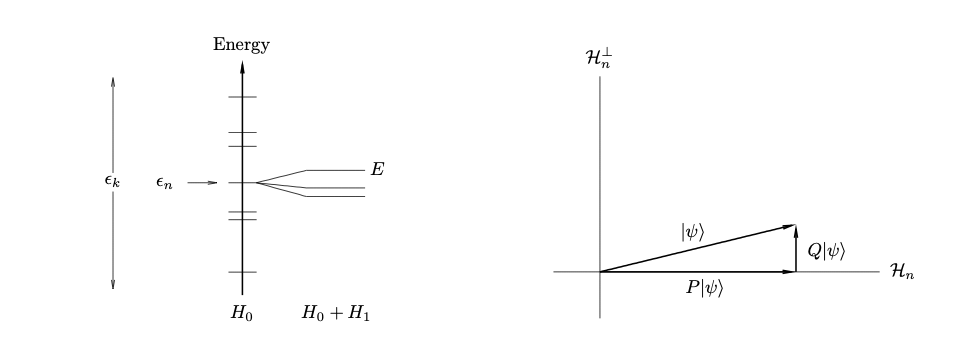
\includegraphics[width=0.8\textwidth]{Figures/QM/LJ_pertTh.png}
    \caption{Algebraic and geometric pictures associated with perturbation
    theory.}
    \label{fig:geoAlgPT}
\end{figure}

It is often true that useful physical systems take the form of a
known system plus a small perturbation; indeed, every prediction
we see from colliders like the LHC tacitly assume this statement.
So we should have a formalism to deal with these kinds of problems; 
this is the study of \vocab{perturbation theory}. We cover the quantum
mechanical version here\footnote{This idea is also found in
classical mechanics and quantum field theory, and more generally
in analysis.}.

Consider a Hamiltonian $H$, and assume that it may be written as
\begin{align*}
    H = H_0 + \lambda H_1 = H_0 + \widetilde{H}_1.
\end{align*}
where $\lambda \in [0, 1]$ interpolates between the free system ($H_0$)
and the full system ($H$). Another way of looking at this is brought to us
by Wilsonian QFT; we may think of $\lambda H_1$ has being an operator
$\widetilde{H}_1 = g \bigo$, where $\bigo$ is composed of $a$'s and $a^\dagger$'s.
Then $\lambda$ is defined through $g = \Lambda^{d - \Delta_\bigo} \lambda$,
with $\Delta_\bigo \coloneqq [\bigo]$ being the mass dimension of $\bigo$,
and we may proceed as usual. As a concrete example, consider the anharmonic 
oscillator---in this case, $H_0 = p^2/2m + (1/2)m\omega^2 q^2$ and 
$\widetilde{H}_1 = g q^4 / 4!$. We have that $\lambda = L^{d - \Delta_\bigo} g$, 
where $L$ is the characteristic length scale of our system, and $d$ the dimension.

We now study the geometry of this problem. Introduce
\begin{align*}
    & \mathcal{H}_n = \{ \text{unperturbed eigenspace} \}
    & \mathcal{H}_n^\perp = \{ \text{perturbed eigenspace} \}.
\end{align*}
These spaces are orthogonal, as they're eigenspaces of different
eigenvalues. Label the kets in the spaces respectively by $\{ \ket{n\alpha} \}$ and 
$\{ \ket{k \alpha} \}$, where $\alpha$ is a label used to resolve 
degeneracies. These states are orthonormal, $\braket{n\alpha}{k\beta} = \delta^{k}_n \delta^{\beta}_\alpha$.
Note that kets correspond to upper indices and bras to lower indices.
Introduce commuting projectors onto the eigenspaces
\begin{align*}
    & P \coloneqq \sum_{\alpha}
    \ketbra{n\alpha}{n\alpha},
    & Q \coloneqq \sum_{\substack{k \neq n \\ \alpha}} \ketbra{k\alpha}{k\alpha}.
\end{align*}
Then $\ket{\psi} = P \ket{\psi} + Q \ket{\psi}$. $P\ket{\psi}$ is known by assumption,
and $Q\ket{\psi}$ is not. This is the goal of perturbation theory: solve for the small hard part
$Q\ket{\psi}$ in terms of big easy part $P\ket{\psi}$. The full Hamiltonian is assumed
to satisfy
\begin{align}
    \label{eq:PTenergyEvals}
    H \ket{\psi} = (H_0 + \lambda H_1)\ket{\psi} = E \ket{\psi},
\end{align}
where $E$ and $\ket{\psi}$ are assumed to be $\lambda$-dependent. As $\lambda \to 0$,
$E \to \epsilon_n$ and $\ket{\psi} \to \ket{n\alpha} \in \mathcal{H}_n$. This second
statement shows the difficulty of degenerate perturbation theory; since $\mathcal{H}_n$
is degenerate, the ``tracing back'' of $\ket{\psi}$ as $\lambda$ turns off is not unique,
and this is also true in reverse---as we turn on $\lambda$, $\ket{\psi}$ generically splits
into one of many energy eigenstates, the number of which determined by $\dim{\mathcal{H}_n}$.

As stated before, we may write $\ket{\psi} = P\ket{\psi} + Q\ket{\psi}$,
where the perturbation is entirely found in $Q\ket{\psi}$. Rewriting eq. 
(\ref{eq:PTenergyEvals}) gives
\begin{align}
    \label{eq:PTEminusH0}
    (E - H_0)\ket{\psi} = \lambda H_1 \ket{\psi}.
\end{align}
So, we'd like to invert $E - H_0$. Write $E - H_0$ as a
function of the energy eigenstates,
\begin{align*}
    E - H_0 = \sum_{k, \, \alpha} \frac{\ketbra{k\alpha}{k\alpha}}{E - \epsilon_k}.
\end{align*}
This expression has a zero eigenvalue at $E = \epsilon_n$, and so it
is meaningless as it stands. To resolve this, introduce
\begin{align*}
    R = \sum_{\substack{k \neq n\\ \alpha}} \frac{\ketbra{k\alpha}{k\alpha}}{E - \epsilon_k}.
\end{align*}
$R$ satisfies $RQ = QR = R$, and $[R, P] = 0$. We also note that $R (E - H_0) = (E - H_0)R = Q$,
and so $R|_{\mathcal{H}_n^\perp} = \id_{\mathcal{H}_n^\perp}$, and $Q\ket{\psi} = \lambda R H_1 \ket{\psi}$
(which we can see by multiplying (\ref{eq:PTEminusH0}) through by $R$). So,
\begin{align*}
    \ket{\psi} = P \ket{\psi} + Q \ket{\psi} = P \ket{\psi} + \lambda R H_1 \ket{\psi}.
\end{align*}
Solving for $\ket{\psi}$ and expanding gives
\begin{align}
    \label{eq:PTstate}
    (1 - \lambda R H_1) \ket{\psi} = P \ket{\psi} \implies \boxed{\ket{\psi} = \sum_{n = 0}^\infty \lambda^n (RH_1)^n P \ket{\psi}.}
\end{align}
So we've accomplished our goal of writing $\ket{\psi}$ in
terms of the easy part $P\ket{\psi}$. We now explore the consequences
of this equation with a few general examples.

\begin{eexample}
    [Non-degenerate perturbation theory]
    Assume $\dim{\mathcal{H}_n} = 1$---call this state $\ket{n}$. Note that
    $\braket{\psi}{n} = 1$ by assumption of $\braket{n}{n} = 1$. $P$ takes an
    especially simple form in this case, $P = \ketbra{n}{n}$. Referencing eq. (\ref{eq:PTstate}),
    we have
    \begin{align*}
        \ket{\psi} & = \ket{n} + \lambda R H_1 \ket{n} + \lambda^2 (RH_1)^2 \ket{n} + \cdots\\
        & = \ket{n} + \sum_{\substack{k \neq n \\ \alpha}} \ket{k\alpha} \frac{\bra{k\alpha}H_1 \ket{n}}{E - \epsilon_k} + \cdots
    \end{align*}
    The energies are given by bra-ing through eq. (\ref{eq:PTEminusH0})
    by $\bra{n}$,
    \begin{align*}
        \bra{n}E - H_0 \ket{\psi} = E - \epsilon_n = \lambda \bra{n} H_1 \ket{\psi},
    \end{align*}
    so
    \begin{align*}
        E = \epsilon_n + \lambda \bra{n} H_1 \ket{n} + \lambda^2 \bra{n} H_1 R H_1 \ket{n} + \cdots
    \end{align*}
    Substituting the zeroth-order approximation for $E$ ($E = \epsilon_n$) gives
    \begin{align*}
        \ket{\psi} = \ket{n} + \lambda \sum_{\substack{k \neq n \\ \alpha}} \ket{k\alpha} \frac{\bra{k\alpha}H_1 \ket{n}}{\epsilon_n - \epsilon_k} + \cdots
    \end{align*}
    which, along with the equation for $\ket{\psi}$, agrees with RSPT to first order.
    We remark upon a general fact here: the $\lambda$-expansion for $E$ is always ``one-behind''
    the expansion for $\ket{\psi}$. Concretely, if we know $E$ to order $\lambda^n$,
    then we know $\ket{\psi}$ to order $\lambda^{n + 1}$. This is because $E$ only shows
    up in $\ket{\psi}$ \emph{starting at} order $\lambda$, so $\ket{\psi}$ is always
    ``one-ahead'' of $E(\lambda)$. 

    In RSPT, we simply identify things slightly differently.
    $\ket{n} \to \ket{n_0}$, and $\lambda^k (RH_1)^k \ket{n} \to \ket{n_k}$.
    Each of the states $\{ n_k \}$ is assumed to be orthogonal to $\ket{n_0}$,
    which follows from the fact that $R$ projects out all $k = n$ states,
    or from using eq. (\ref{eq:PTEminusH0}) and noting that that $\braket{P\psi}{Q\psi} = 0$.
    Everything else follows from this.
\end{eexample}

\begin{eexample}
    [Degenerate perturbation theory]
    We assume that the unperturbed eigenspace is degenerate,
    and thus $P = \sum_\alpha \ketbra{n\alpha}{n\alpha}$.
    $P$ acting on $\ket{\psi}$ gives some combination of
    the $\ket{n\alpha}$'s, $P\ket{\psi} = \sum_\alpha c_\alpha \ket{n\alpha}$.
    The main difference between non-degenerate and degenerate
    perturbation theory is that we must solve for the state ($c_\alpha$)
    and the energy $E$ simultaneously. Subbing $\ket{\psi}$ into the energy
    equation we previously found gives
    \begin{align*}
        & \text{\underline{State}:} & \ket{\psi} = c_\alpha \ket{n\alpha} + \lambda R H_1 (c_\alpha \ket{n\alpha}) + \cdots\\
        & \text{\underline{Energies}:} & (E - \epsilon_n) c_\alpha = \left\{ \lambda \ket{n\alpha}H_1 \ket{n\beta} + \lambda^2 \sum_{\substack{k \neq n \\ \gamma}} \frac{\bra{n\alpha} H_1 \ket{k\gamma} \bra{k\gamma} H_1 \ket{n\beta}}{E - \epsilon_k} + \cdots \right\} c_\beta.
    \end{align*}
    From the second equation we can see what the $c_\alpha$'s are:
    eigenvectors with respect to the $g \times g$ matrix in the braces
    (with $g = \dim{\mathcal{H}_n}$). Their eigenvalues are $(E - \epsilon_n)$.
    In practice, we truncate the energy series at $\bigo(\lambda)$.

    \note{show equivalence to RSPT}
\end{eexample}

\begin{eexample}
    [Nearly degenerate perturbation theory]
\end{eexample}







\subsubsection{Lagrangian}

\end{document}